% Re-defined by Z.C.TIAN (https://github.com/doem97)
% This version comply with the Official EEE Dissertation Guidline in (https://eeen40028.eee.ntu.edu.sg/graduate/forms/Coursework/Student/PDFs/Guidelines/Diss_Guideline.pdf)
% More information about dissertation can be found in (https://eeen40028.eee.ntu.edu.sg/graduate/index.htm)
% Based on W.M.ZHAO version, original link in overleaf:
% (https://www.overleaf.com/latex/templates/ntu-master-dissertation/ngnhrrwryccv)

\documentclass[12pt]{report}

%% Useful packages
\usepackage[a4paper,top=3cm,bottom=3cm,left=3.5cm,right=3cm,marginparwidth=1.75cm,headheight=22pt]{geometry}
\usepackage{amsmath}
\usepackage{cite}
\usepackage{courier}
\usepackage[export]{adjustbox}
\usepackage[labelfont=bf, textfont=bf]{caption}
\usepackage{graphicx}
\usepackage{hyperref}
\usepackage{float}
\usepackage{setspace}
\usepackage{subfigure}
\usepackage{setspace}
\usepackage{lipsum}
\usepackage{fancyhdr} % Fancy header
\usepackage{url}
\usepackage{tabularx}
\usepackage[utf8]{inputenc}
\usepackage{mathptmx} %Times Font
\usepackage{placeins}
\usepackage{graphicx}
\usepackage[toc]{appendix}

\usepackage{listings}
\usepackage{color}
\definecolor{eclipseBlue}{RGB}{42,0.0,255}
\definecolor{eclipseGreen}{RGB}{63,127,95}

\lstset {
  basicstyle=\small\ttfamily,
  captionpos=b,
  tabsize=2,
  columns=fixed,
  breaklines=true,
  frame=l,
  numbers=left,
  numberstyle=\small\ttfamily,
  morekeywords= {
    EQUAL, GREATER, LESS, NONE, SOME, abstraction, abstype, and, andalso, array, as, before, bool, case, char, datatype, do, else, end, eqtype, exception, exn, false, fn, fun, functor, handle, if, in, include, infix, infixr, int, let, list, local, nil, nonfix, not, o, of, op, open, option, orelse, overload, print, raise, real, rec, ref, sharing, sig, signature, string, struct, structure, substring, then, true, type, unit, val, vector, where, while, with, withtype, word
  },
  morestring=[b]",
  morecomment=[s]{(*}{*)},
  stringstyle=\color{black},
  identifierstyle=\color{eclipseBlue},
  keywordstyle=\color{red},
  commentstyle=\color{eclipseGreen}
}

%==== Header and Footer configure ====
% Define the plain pagestyle used by most chapters
\fancypagestyle{plain}{
\fancyhf{} % Clear header footer
\fancyhead[R]{\bf \textsl{\leftmark} \vspace{0.1in}}
\fancyfoot[R]{\thepage}
% Set the right side of the footer to be the page number
\renewcommand{\headrulewidth}{2pt}
}
% For those Chapter* (Can't use \leftmark to call their chapter name directly)
\fancypagestyle{addin}{
\fancyhf{} % Clear header footer
\fancyhead[R]{\bf \textsl{\leftmark} \vspace{0.1in}}
% Set the right side of the footer to be the page number
\fancyfoot[R]{\thepage}
\renewcommand{\headrulewidth}{2pt}
}

%==== Overall Config ====
\setlength{\parindent}{0in} % Set paragraph indent as 0
% \setlength{\fboxsep}{-0.3in}%
\setlength{\fboxrule}{0.5pt} % Set the bounding box around the image as 0.5pt
\pagestyle{plain}



\begin{document}
\fontdimen2\font=0.5em% inter word space
%==== FRONT PART====
\begin{titlepage}

\vspace{3in}

\centering
\Huge{\textbf{Modelarea Proceselor\\din Cadrul unei Companii}}\\[2in]

\LARGE{\textbf{Nistor Marian-Sergiu\\Sescu Alexandra}}\\[0.5in]

\end{titlepage}
\newpage % Coverpage
%\include{Title/titlepage} % Titlepage
%\include{Title/SoO} % SoO
%\include{Title/SDS} % SDS
%\include{Title/AAS} % AAS

%\begingroup
%\let\cleardoublepage\clearpage

\pagenumbering{roman}

\renewcommand*\contentsname{\centering Table of Contents}
\tableofcontents
\newpage

%\endgroup

%==== MAIN PART ====

\pagenumbering{arabic}
%=== CHAPTER ONE (1) ===
%=== SPECIFICATIILE PROIECTULUI ===

\chapter{Specificatiile proiectului}
\begin{spacing}{1.5}
\setlength{\parskip}{0.3in}

Obiectivul proiectului consta in modelarea proceselor din cadrul unei companii bazate pe mai multe module:
\begin{itemize}
\item Modulul "HQ", care coordoneaza departamentele
\item Modulul "Shop", in cadrul caruia se genereaza si se comercializeaza produse
\item Modulul "Localization", care trateaza localizarea clientilor, pe baza informatiei primite de la sateliti de GPS, in scopul transportului produsului cerut
\item Modulul "Shipment", in cadrul caruia produsul este transportat si predat clientului
\item Modulul "Customer Service", care asigneaza un agent unei reclamatii primite din partea unui client, in urma unei livrari
\item Modulul "Marketing", care serveste gasirea noilor clienti, prin organizarea campaniilor de marketing.
\end{itemize}

\section{Modulul "HQ"}

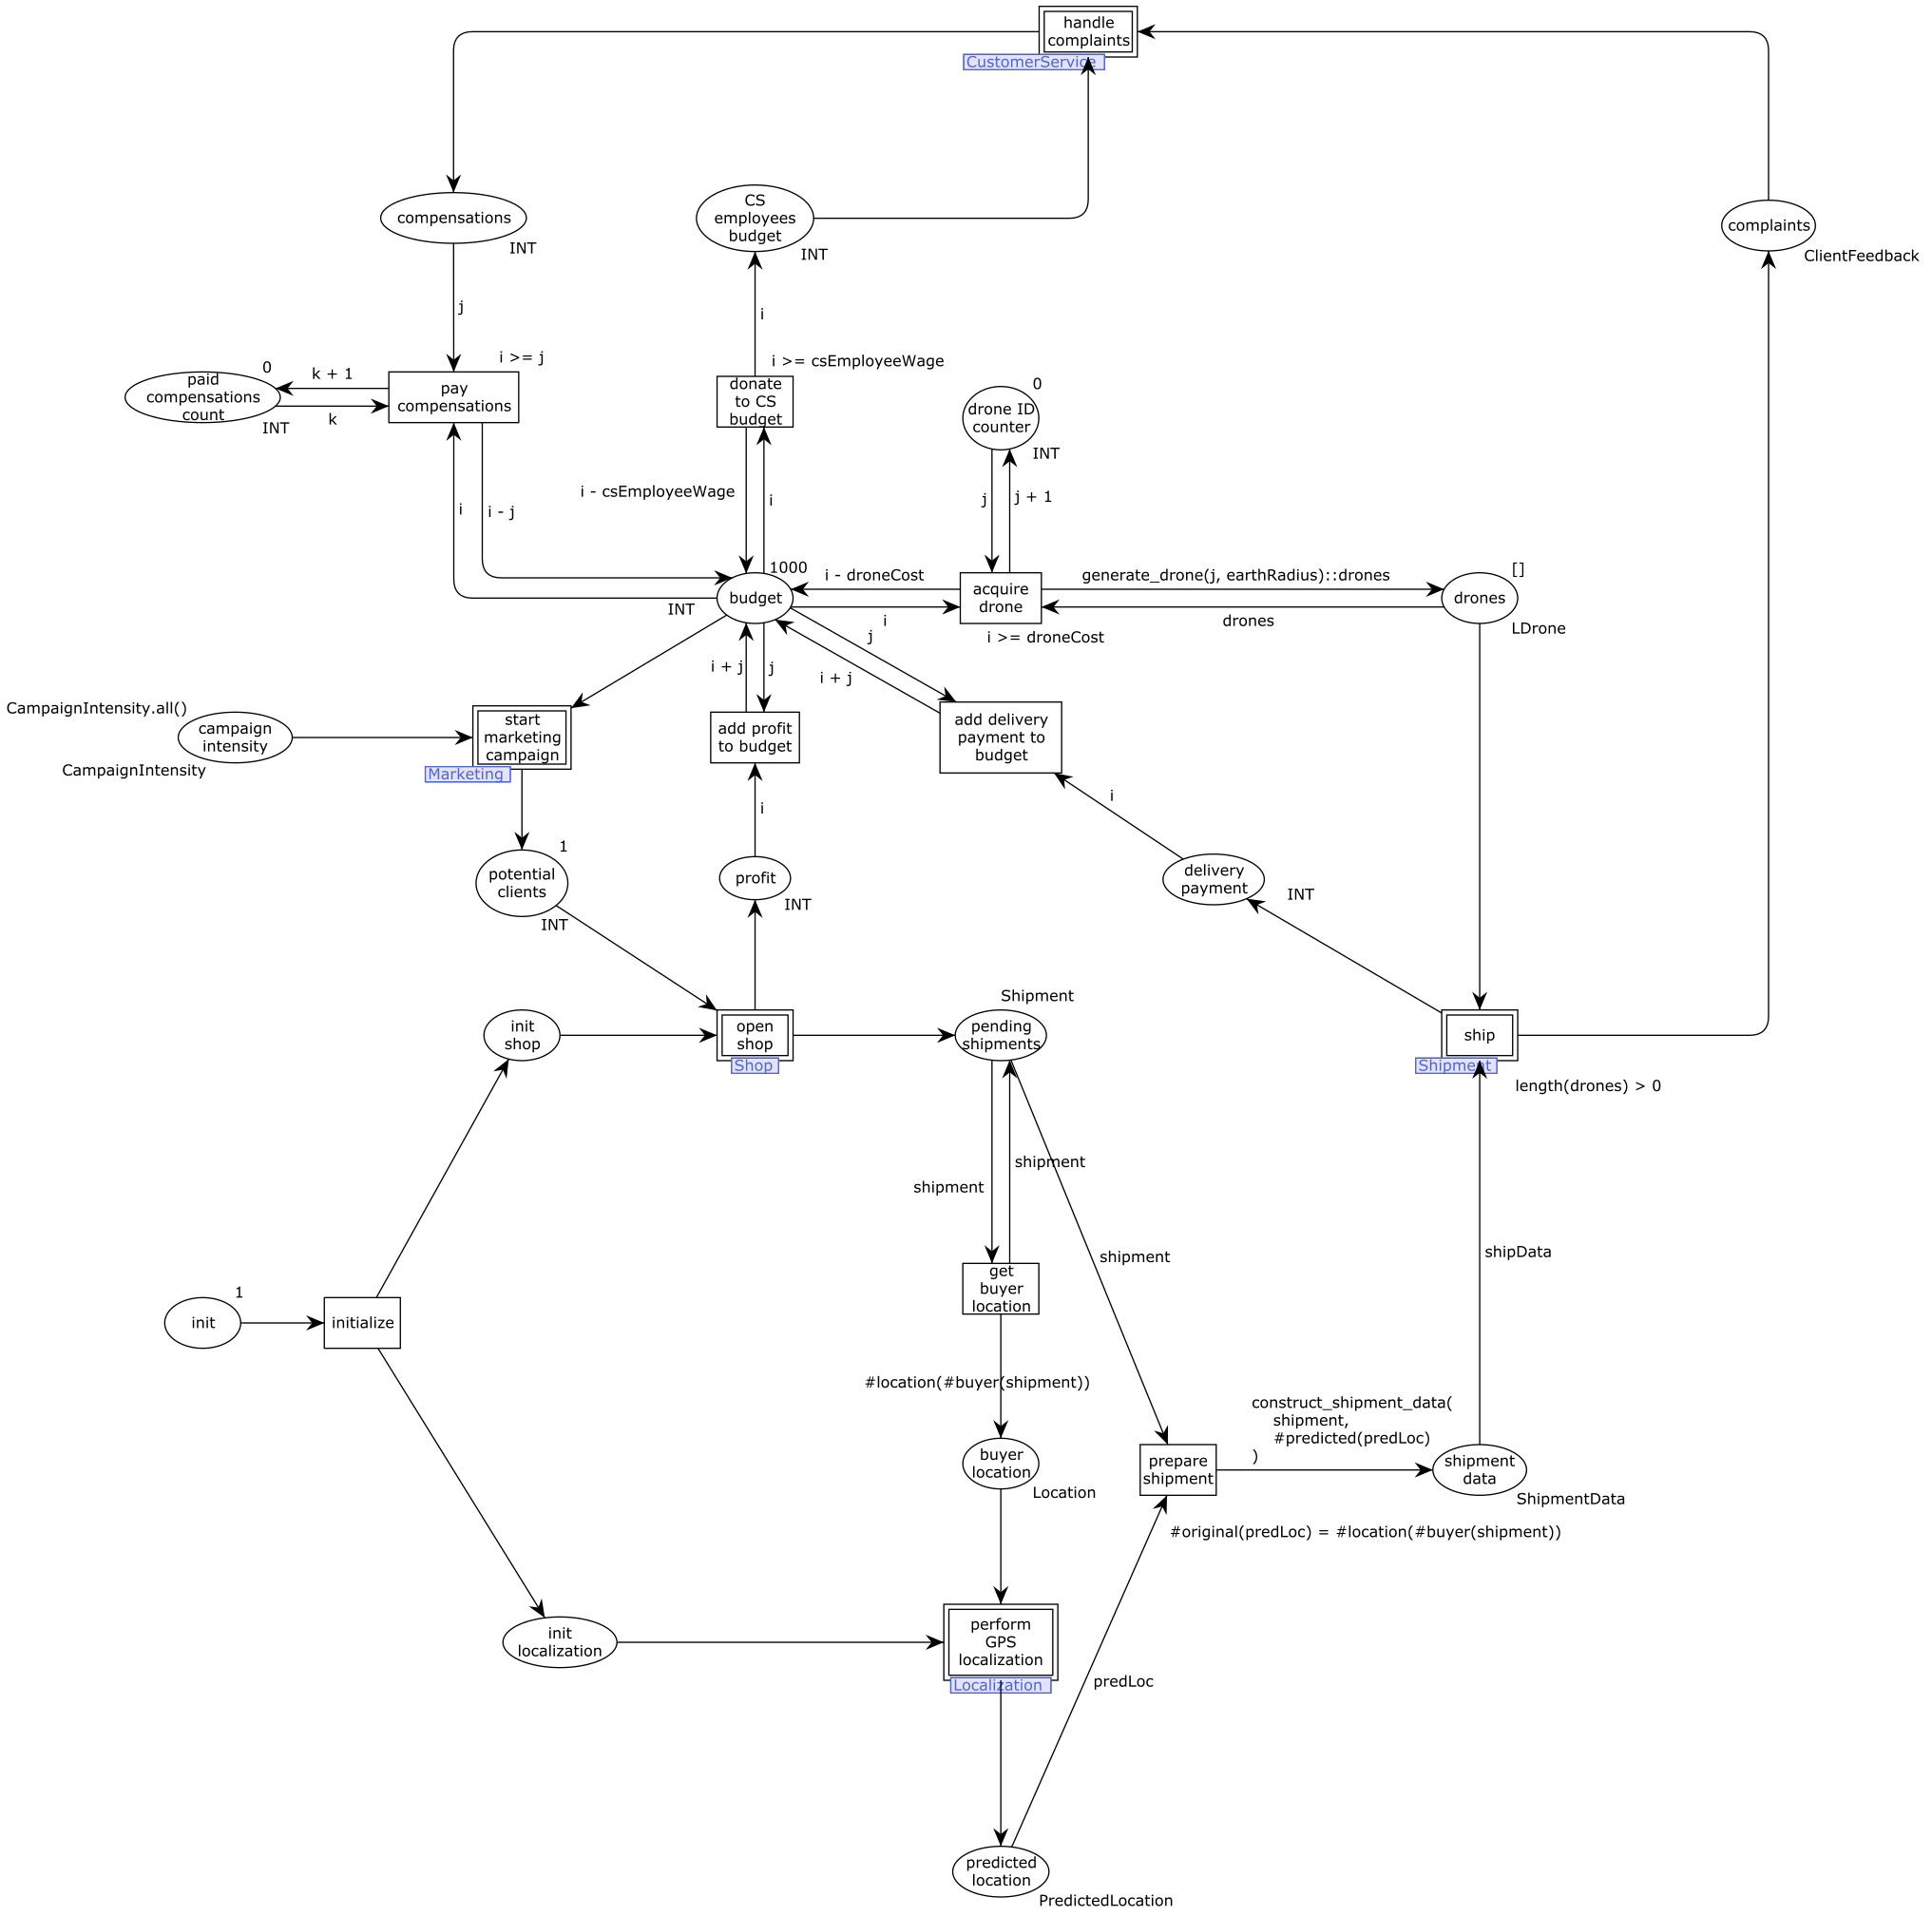
\includegraphics[width=\textwidth]{./Parts/Chapter1/HQ.png}

Modulul "HQ" are ca scop coordonarea departamentelor din cadrul companiei.\\
In primul rand, din starea $init$ se realizeaza tranzitia $initialize$, activand componentele "Shop" si
"Localization".\\
In urma realizarii unei vanzari in cadrul modulului "Shop", se plaseaza profitul in starea $profit$, care
apoi se poate adauga la bugetul companiei, situat in starea $budget$, prin tranzitia $add\ profit\ to\ budget$.
Pentru fiecare tranzactie, componenta "Shop" adauga o entitate de tip $Shipment$, in starea
$pending\ shipments$. Prin tranzitia $get\ buyer\ location$ se plaseaza locatia cumparatorului in
$buyer\ location$, fiind input pentru modulul "Localization". Locatia reala a clientului nu ar fi cunoscuta
inainte de localizarea GPS, insa este reprezentata in cadrul retelei, in scop demonstrativ.\\
In urma localizarii clientului, in starea $predicted\ location$ se vor gasi coordonatele aproximative ale
cumparatorului. Entitatea de tip $Shipment$, situata in $pending\ shipments$ este concatenata cu locatia
prezisa a clientului, returnand datele despre transport, in forma lor finala, in starea $shipment\ data$,
prin tranzitia $prepare\ shipment$.\\
Apoi, modulul de "Shipment" realizeaza livrarea, plasand in $delivery\ payment$ plata transportului, achitata
de cumparatorul produsului. Transportul se realizeaza cu ajutorul dronelor, situate in starea $drones$,
care pot fi cumparate prin tranzitia $acquire\ drone$, daca permite bugetul companiei.\\
In urma livrarii, clientul poate face o reclamatie, stocata cu tipul $ClientFeedback$, in starea $complaints$.
Reclamatiile sunt tratate de componenta "Customer Service". Agentii de customer service pot fi platiti prin
tranzitia $donate\ to\ CS\ budget$, cu o suma prestabilita. In urma tratarii neintelegerii cu clientul,
acesta va primi o compensatie din partea companiei, platita prin intermediul tranzitiei $pay\ compensations$.\\
Pentru a gasi clienti noi, firma poate incepe o campanie de marketing, in cadrul modulului "Marketing".
Clientii noi vor fi plasati in starea $potential\ clients$.

\section{Modulul "Shop"}

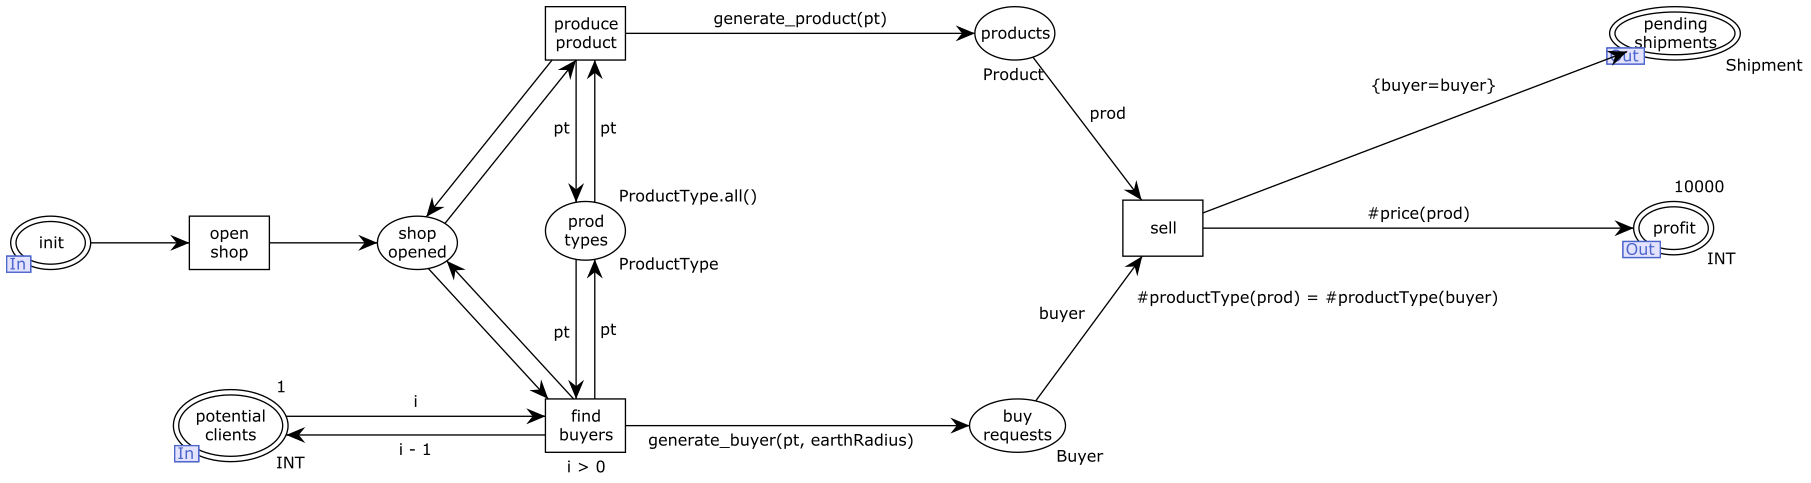
\includegraphics[width=\textwidth]{./Parts/Chapter1/Shop.png}

Modulul "Shop" are ca scop generarea si comercializarea produselor oferite de companie.\\
Mai intai, prin intermediul tranzitiei $open\ shop$, devine posibila generarea de noi produse si
identificarea noilor clienti. Produsele sunt plasate in starea $products$, iar cumparatorii, in
$buy\ requests$. Fiecarui produs i se atribuie un pret aleatoriu, generat pe baza unei distributii normale.
Locatia clientilor este generata, de asemenea, aleatoriu. Latitudinea si longitudinea urmeaza distributii
uniforme. Fiecare cumparator poate fi asociat cu un anumit tip de produs. In urma realizarii unei astfel de
asocieri, prin tranzitia $sell$, se plaseaza noua livrare, in starea de output $pending\ shipments$.
Profitul obtinut de companie se va afla in starea de output $profit$, urmand ca acesta sa fie adaugat la
buget.

\section{Modulul "Localization"}

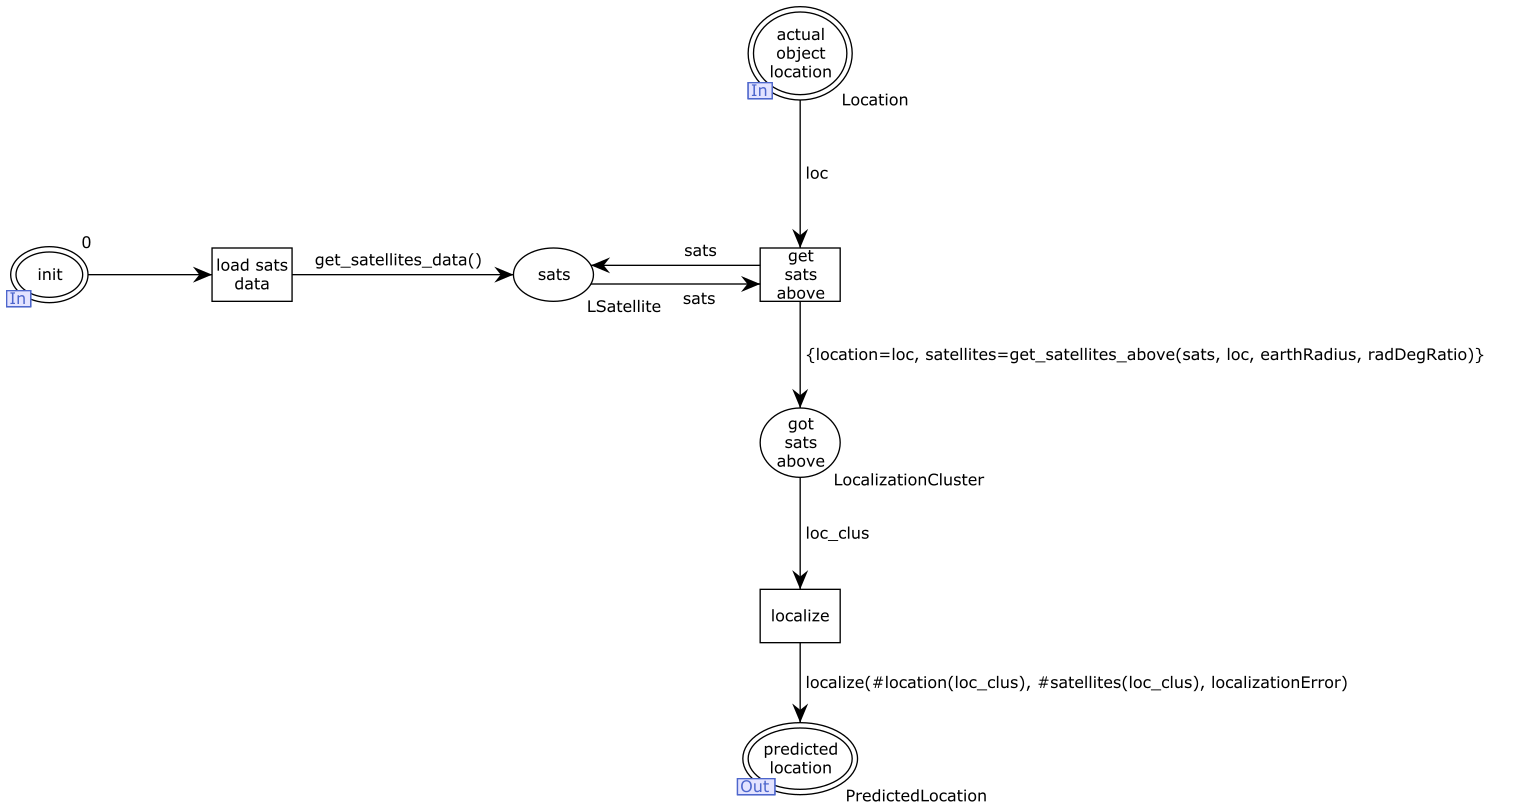
\includegraphics[width=\textwidth]{./Parts/Chapter1/Localization.png}

Scopul modulului "Localization" este de a identifica locatia aproximativa a clientilor, pe baza satelitilor
GPS.\\
Datele despre sateliti sunt returnate de functia $get\_satellites\_data$, generata automat in fisierul sursa
"satellites\_data.sml", creat cu ajutorul scriptului "get\_satellites\_data.py". Sunt stocate informatii
reale despre pozitia satelitilor de GPS care orbiteaza in jurul Pamantului (latitudine, longitudine,
altitudine).\\
Locatiile satelitilor sunt plasate in starea $sats$, prin intermediul tranzitiei $load\ sats\ data$.
Considerand locatia clientului (prezenta in $actual\ object\ location$, in scop demonstrativ), se sustrag
satelitii aflati deasupra sa, doar acestia fiind capabili sa il localizeze. In urma executiei tranzitiei
$localize$, satelitii de GPS aproximeaza locatia cumparatorului, plasand-o in starea de output
$predicted\ location$. Aproximarea este supusa unei eroari generate aleatoriu uniform, per fiecare satelit.

\section{Modulul "Shipment"}

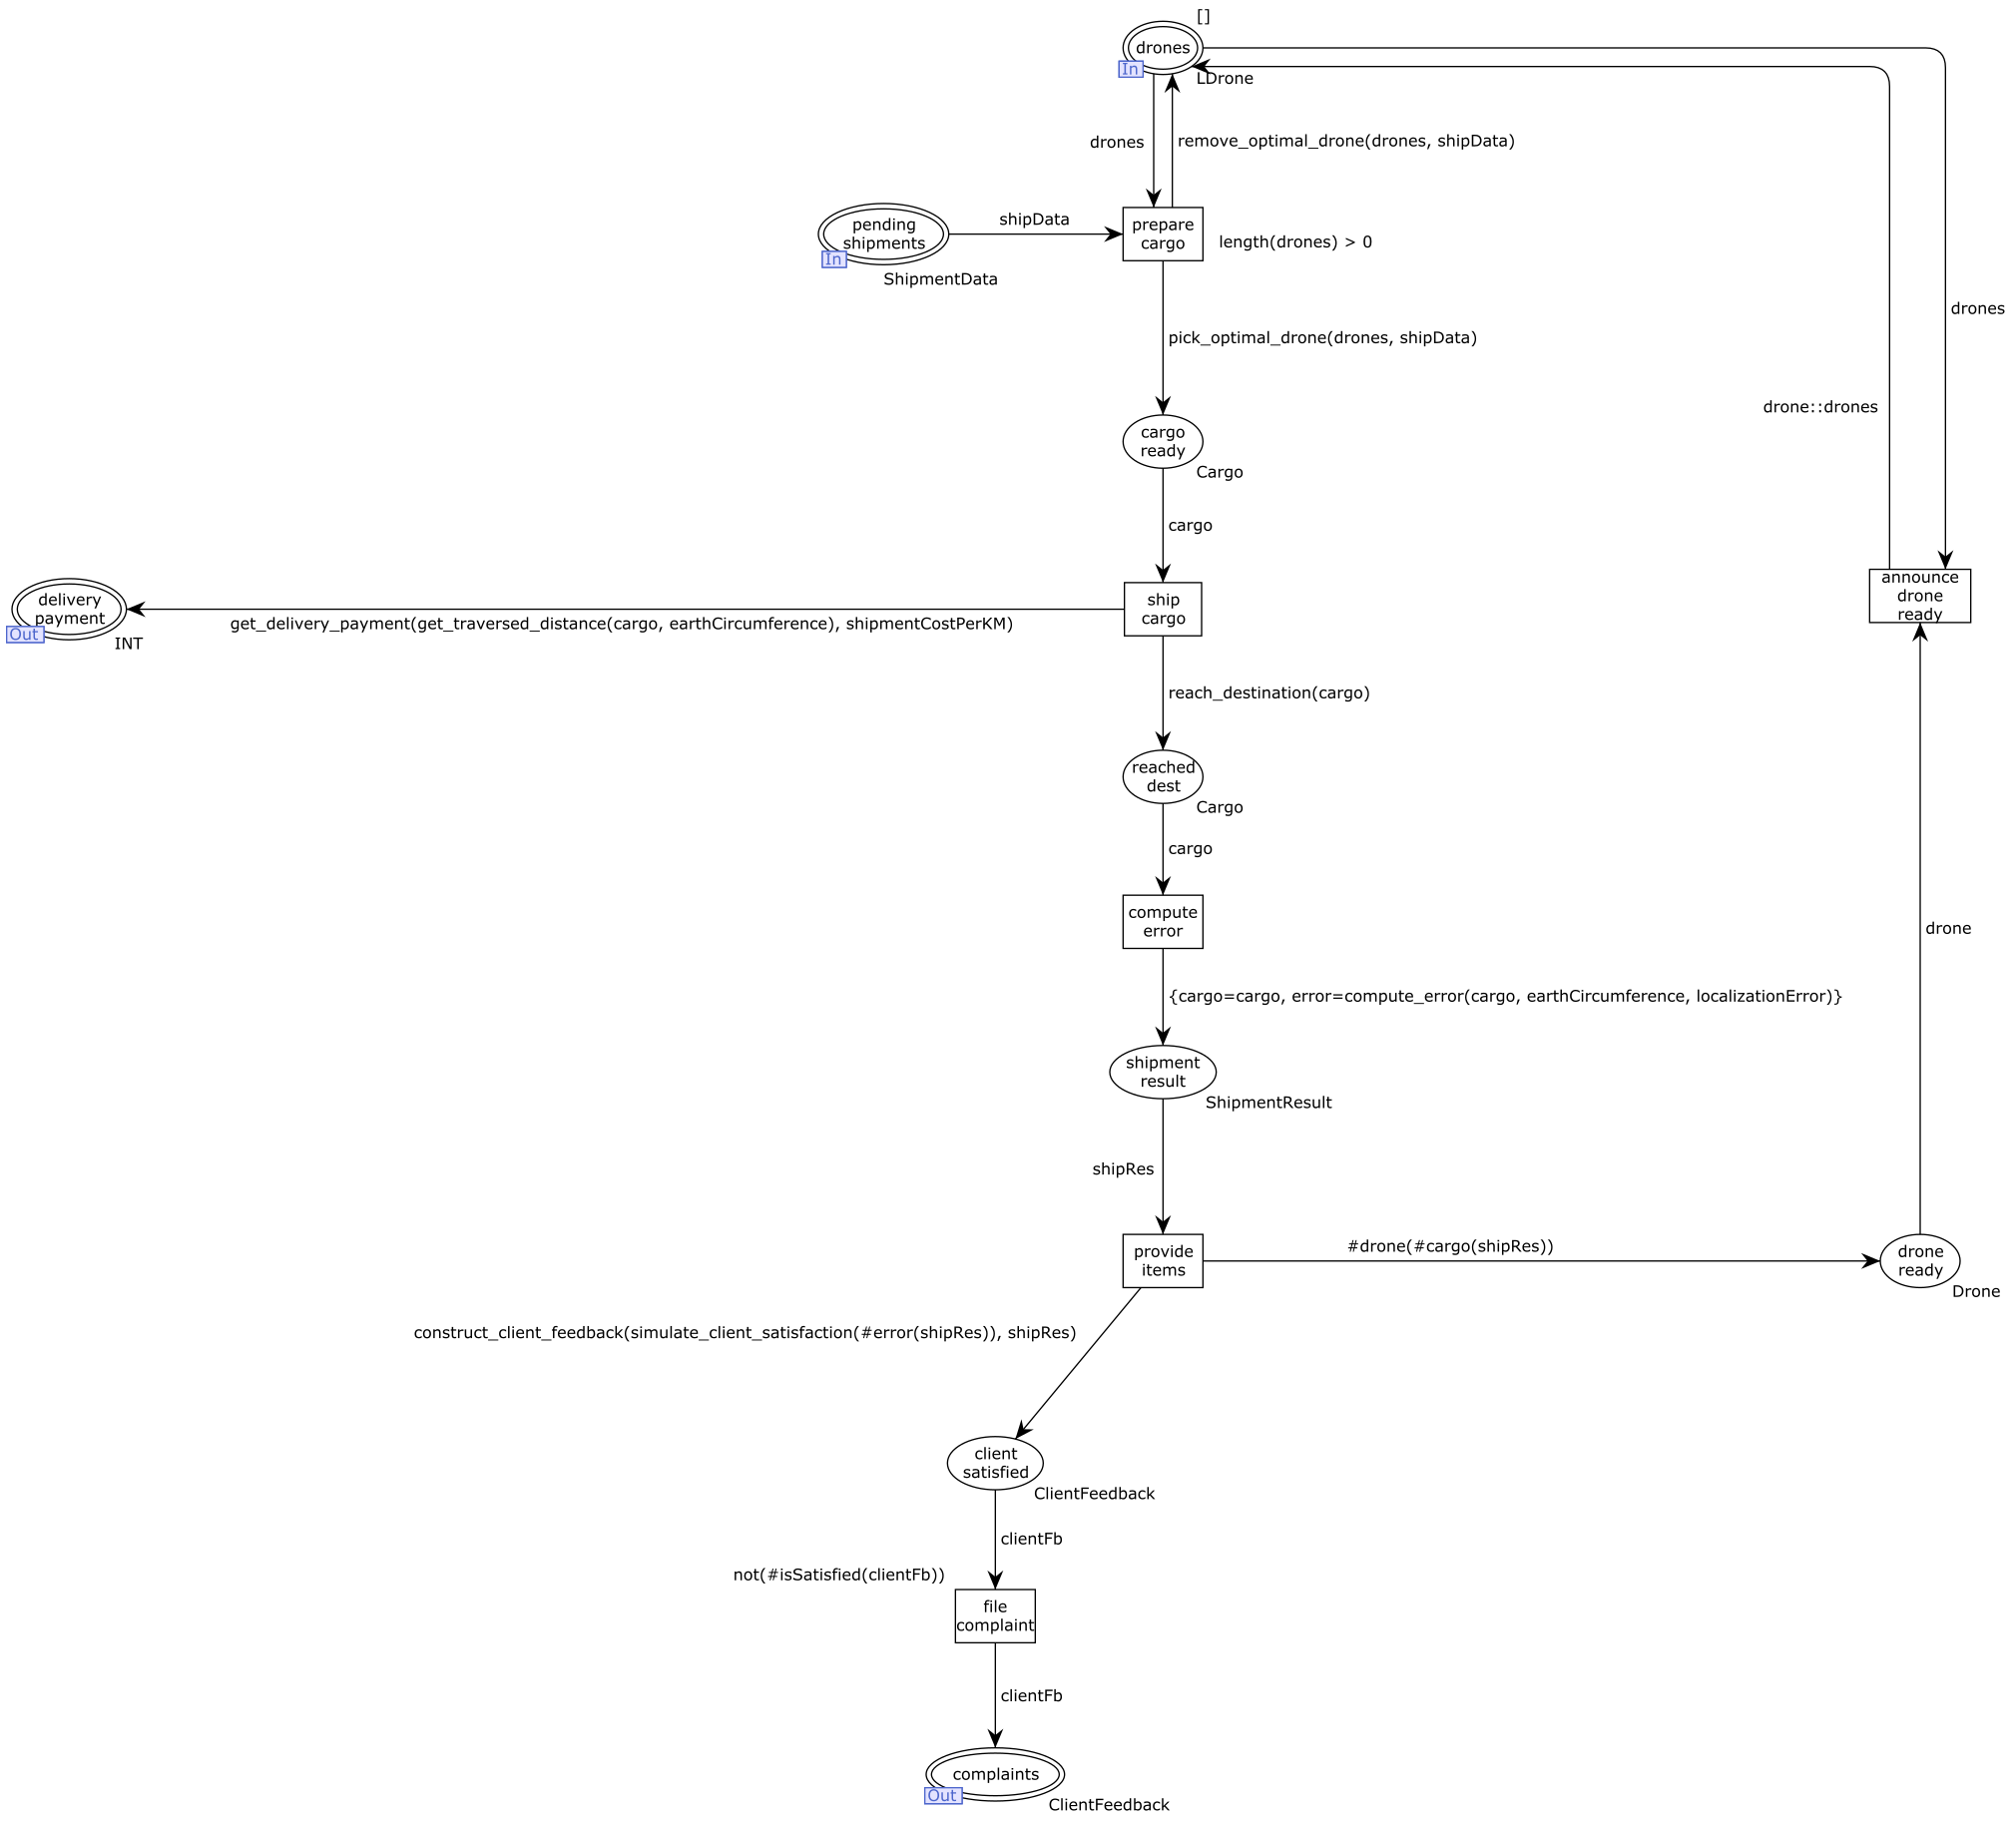
\includegraphics[width=\textwidth]{./Parts/Chapter1/Shipment.png}

Modulul "Shipment" trateaza livrarea produselor catre client, cu ajutorul dronelor.\\
Locatiile de input pentru aceasta componenta sunt $pending\ shipments$ si $drones$, continand date
referitoare la transport si o lista cu dronele disponibile. In urma tranzitiei $prepare\ cargo$, se asigneaza
drona cea mai apropiata de client, generandu-se o entitate de tip $Cargo$. In cadrul tranzitiei $ship\ cargo$
se calculeaza pozitia finala a dronei. Pozitia finala depinde de eroarea rezultata din aproximarea pozitiei
cumparatorului, in modulul "Localization". De asemenea, se calculeaza costul transportului, suma platita
de client fiind stocata in locatia de output $delivery\ payment$, urmand ca aceasta sa fie adaugata
la bugetul companiei. Eroarea este calculata in cadrul tranzitiei $compute\ error$, plasand rezultatul
transportului in $shipment\ result$. In urma executiei actiunii $provide\ items$, drona este stocata in
$drone\ ready$, urmand ca aceasta sa fie readaugata in locatia $drones$, prin tranzitia
$announce\ drone\ ready$. Feedback-ul clientului este stocat in starea $client\ satisfied$.
Acesta depinde de eroarea in aproximarea locatiei in care este livrat produsul. In cazul in care
clientul este nemultumit, acesta poate trimite o reclamatie companiei, prin $file\ complaint$.
Reclamatiile vor fi tratate de echipa "Customer Service".

\section{Modulul "Customer Service"}

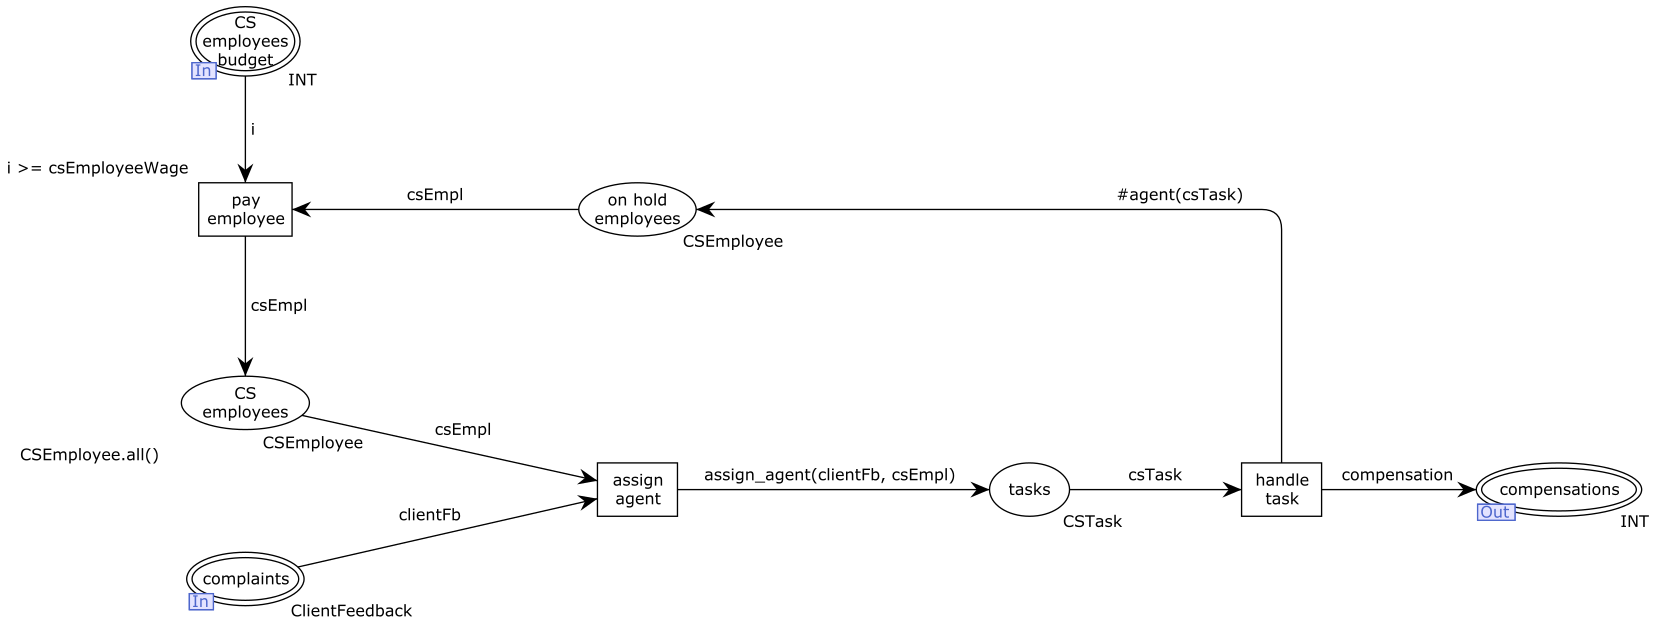
\includegraphics[width=\textwidth]{./Parts/Chapter1/CustomerService.png}

Modulul "Customer Service" trateaza reclamatiile primite de la clienti in urma livrarilor.\\
Reclamatiile vor fi stocate in locatia $complaints$. Daca sunt agenti disponibili in $CS\ employees$,
se asigneaza unul dintre ei respectivei reclamatii, prin tranzitia $assign\ agent$, generandu-se in $tasks$
o entitate de tip $CSTask$. In urma tratarii unui task, clientului i se promite o compensatie, care va fi
achitata, pe baza bugetului companiei, in modulul "HQ". Dupa finalizarea unui task, angajatul este plasat
in locatia $on\ hold\ employees$. Bugetul asignat agentilor de customer service se afla in starea de input
$CS\ employees\ budget$. Angajatul nu va fi disponibil pentru a trata o alta reclamatie pana cand nu este
platit de catre companie, prin tranzitia $pay\ employee$.

\section{Modulul "Marketing"}

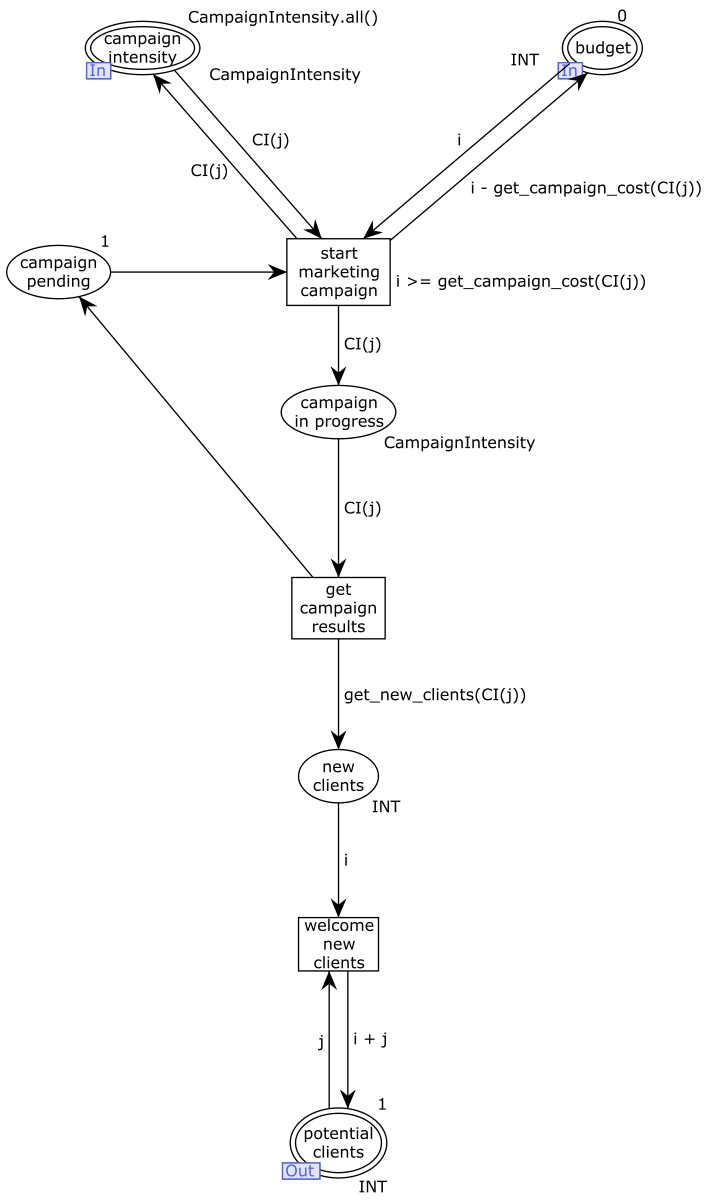
\includegraphics[width=0.8\textwidth]{./Parts/Chapter1/Marketing.png}

Scopul modulului de "Marketing" este atragerea noilor clienti, in urma campaniilor de marketing.\\
O singura campanie poate fi activa la un moment dat. Locatia $campaign\ pending$ asigura acest fapt.
In urma executiei tranzitiei $start\ marketing\ campaign$, o noua campanie este initializata. Intensitatea
unei campanii determina numarul de clienti care vor fi convinsi spre a cumpara produsele companiei. Campaniile
mai eficiente vor implica cheltuieli mai mari din partea companiei.
Prin executia tranzitiei $get\ campaign\ results$, se plaseaza numarul de clienti noi in locatia $new\ clients$,
acest numar fiind calculat pe baza unei distributii uniforme. Actiunea $welcome\ new\ clients$ adauga noii
client in $potential\ clients$, aceasta fiind locatie input pentru modulul "Shop".

\end{spacing}
%=== END OF CHAPTER ONE ===
\newpage



%=== CHAPTER TWO (2) ===
%=== DECLARATIONS ===

\chapter{Declaratii} 
\begin{spacing}{1.5}
\setlength{\parskip}{0.3in}

\section{Colset-uri}

\section{Variabile}

\section{Constante}

\section{Functii}

\end{spacing}
%=== END OF CHAPTER TWO ===
\newpage




%==== ENDING PART ===
%==== END OF ALL ===
\end{document}